\documentclass[11pt,a4paper]{article}

\usepackage[margin=1in]{geometry}
\usepackage[hidelinks]{hyperref}
\usepackage{graphicx}

\setlength{\parindent}{0pt}
\setlength{\parskip}{0.6em}

\title{AI651 - Assignment 1}
\author{\textit{[Amna Kharral]} \quad \textit{[25280047]}}
\date{}

\begin{document}
\maketitle

\textbf{Code repository:} \textit{[https://github.com/amorde-ccg-20/PA1-DLSTG]}

\section*{Task 1: Forecasting Across Heterogeneous Sensors}
\subsection*{Response 1A: Predict and Check the Overall Model Ranking}

\subsubsection*{Initial prediction before Output 1.1}

% Predicted order retained; wording revised for clarity.

For stations 1-3, which are used to train the models, I expect the models to
rank as follows, from lowest to highest forecast error:
\begin{center}
Period-routed ridge $\rightarrow$ Raw Attention $\rightarrow$
Sensor-specific ridge $\rightarrow$ Shared ridge
\end{center}

A station's vibration can repeat faster or slower over time. Period-routed
ridge estimates how many time steps one cycle takes in the recent readings.
It then uses a ridge model fitted to readings with a similar cycle length.
The assignment says the simulated signal contains a repeating vibration
cycle, so this should help when the cycle length is estimated accurately.

Raw Attention uses the recent readings to decide which earlier readings to
focus on. This may help it adjust when the vibration speeds up or slows down.
It also has to learn the repeating cycle while handling the slowly changing
baseline, so I do not expect it to beat a model that estimates the cycle length
directly.

Giving each known station its own ridge model might help because stations
differ slightly. But each model learns from less data, and it still uses the
same rule when that station's operating speed changes. So the expected
improvement is uncertain.

Station 4 is kept out of training. For this station, I expect:
\begin{center}
Period-routed ridge $\rightarrow$ Raw Attention $\rightarrow$ Shared ridge
\end{center}

All three models can use station 4's recent readings. The same operating speed
ranges apply to every station, so the period-routed model may also work here.
Sensor-specific ridge cannot be used: it needs a separate model fitted to each
station, and none was fitted to station 4.

\clearpage
\subsubsection*{Measured comparison and revision: Output 1.1}

The results below use the \texttt{full} preset, data seed 0, and model seed 0.
They come from the validation split. Raw Attention was trained for
6,000 steps. The predicted order above has not changed.

\begin{table}[ht]
\centering
\small
\setlength{\tabcolsep}{4pt}
\begin{tabular}{lrrrrrrrr}
\hline
& \multicolumn{4}{c}{Established stations 1-3}
& \multicolumn{4}{c}{Held-out station 4} \\
Model & All & A & B & C & All & A & B & C \\
\hline
Shared ridge & .767 & .805 & .854 & .621 & .876 & .909 & .982 & .713 \\
Sensor-specific ridge & .768 & .804 & .852 & .630 & - & - & - & - \\
Period-routed ridge & .166 & .181 & .164 & .152 & .173 & .184 & .182 & .150 \\
Raw Attention & .431 & .388 & .482 & .418 & .612 & .647 & .580 & .607 \\
\hline
\end{tabular}
\caption{Output 1.1: validation root mean squared error (RMSE) in
$\mathrm{m/s^2}$
A, B and C identify products. Sensor-specific ridge is unavailable for station 4.}
\label{tab:comparison}
\end{table}

\textbf{Overall ranking.}
For stations 1-3, period-routed ridge has the lowest error, followed by Raw
Attention, shared ridge, and sensor-specific ridge. The first two match my
prediction. The last two are reversed and their errors differ by only
$0.0013\,\mathrm{m/s^2}$. Station 4 ranks as: period-routed
ridge, raw attention, and shared ridge.

Compared with shared ridge, period-routed ridge has 78.4\% lower RMSE on
stations 1-3 and 80.3\% lower RMSE on station 4. Raw Attention has 43.8\%
and 30.1\% lower RMSE, respectively. Period-routed ridge also has 61.5\% lower
RMSE than Raw Attention on stations 1-3 and 71.8\% lower RMSE on station 4.


\textbf{Results by product.}
For every product, period-routed ridge has the lowest error and Raw Attention
is second, both on stations 1-3 and on station 4. Sensor-specific ridge is
only slightly better than shared ridge for Products A and B, and worse for C.
Raw Attention's highest product error is on B for stations 1-3 ($0.482$), but
on A for station 4 ($0.647$).

\textbf{Explanation}
Shared ridge and sensor-specific ridge each use the same learned rule when the
vibration speed changes. Splitting the data by station does not solve that
problem, because each station runs at several speeds. Period-routed ridge
estimates the cycle length from the recent readings and chooses a rule for that
speed. It also works well on station 4, which had no station-specific model.
Raw Attention changes what it focuses on for each set of recent readings and
does better than the two fixed-rule models.
These results show that using the current speed helps on this simulated data.


\clearpage
\subsection*{Response 1B: Why Recent Readings Must Shape the Forecast}

\textbf{One fixed rule must handle different speeds (Output 1.2).}
Both validation examples come from station 1. The vibration takes 16.13
samples to repeat under Product A and 30.09 samples under Product C. The
48-step forecast therefore covers about three cycles for A but only 1.6 for
C. The station is the same, but the future peaks are much farther apart for C.

Shared ridge uses $\hat{z}=x^\top\widehat{W}$ for both examples: $x$ is the
recent readings and $\hat{z}$ is the forecast. The forecast changes when $x$
changes, but the learned weights $\widehat{W}$ stay
the same. It cannot switch to a rule fitted for the current speed. Because one
set of weights must handle several speeds, it tends to flatten the cycle in
Figure~\ref{fig:forecasts}. For A, it predicts a peak near 1.1 seconds that is
too low and a following trough that is too high. For C, it flattens the trough
near 1.2 seconds and the peak near 1.8 seconds. The problem is the shape of
the forecast rather than just a vertical shift.

Period-routed ridge follows these peaks and troughs more closely. For these
two examples, shared ridge has RMSE $0.779$ for A and $0.448$ for C, and
period-routed ridge gives even lower numbers at $0.232$ and $0.150$. Raw Attention gives
$0.290$ and $0.378$. These numbers describe the two examples, while
Table~\ref{tab:comparison} averages over all validation windows.

\textbf{Attention changes which readings it uses (Output 1.3).}
For recent readings represented by $X$, one attention head computes
\[
Q=XW_Q,\qquad K=XW_K,\qquad V=XW_V,
\]
\[
A(X)=\mathrm{softmax}\left(\frac{QK^\top}{\sqrt{d_h}}\right),
\qquad \mathrm{output}=A(X)V,
\]
Here $Q$ and $K$ are two views of the readings used to score pairs of time
steps; $V$ holds the information combined using those scores. The number of
features in one head is $d_h$. The learned weights $W_Q$, $W_K$, and $W_V$
stay fixed after training. But new readings change
$Q$ and $K$, which changes the attention weights $A(X)$. The model can then
put more weight on different earlier time steps for each new input.

Figure~\ref{fig:attention} compares the attention weights for the two
station-1 examples. In the first layer, after averaging over heads, the mean
absolute difference between corresponding weights is $0.01128$; the largest
difference is $0.42501$, which shows that attention uses different weights for
different recent readings. 

\clearpage
\begin{figure}[ht]
\centering
\includegraphics[width=\linewidth]{\detokenize{../Question 1/results/design/1.2-1.pdf}}
\caption{Output 1.2: validation forecasts for station 1 under Products A and C.
The dotted line marks where the forecast begins; the black curve shows the
actual future readings.}
\label{fig:forecasts}
\end{figure}

\begin{figure}[ht]
\centering
\includegraphics[width=\linewidth]{\detokenize{../Question 1/results/design/1.3-1.pdf}}
\caption{Output 1.3: first-layer attention weights, averaged over heads, for
the same two sets of recent readings, followed by their difference. Both use
the same trained model}
\label{fig:attention}
\end{figure}

\clearpage
\subsection*{Response 2: Separate Slow Changes from Repeating Vibration}

\textbf{What the split does (Output 2.1).}
The moving average estimates the slow part $T$ from nearby readings. The
remaining part is $x-T$, so the method returns $(x-T,T)$. Near the start or end of the
input, the averaging window needs readings that do not exist. We fill those positions by 
repeating the first or last available reading. We selected an averaging width of \textbf{41 samples}.
In the station-2, Product-C example in Figure~\ref{fig:decomposition}, width
17 follows some of the fast vibration, leaving a weaker cycle in $x-T$.
Width 41 follows the slow rise and leaves a clearer cycle: the standard
deviation of $x-T$ rises from $0.578$ to $1.572\,\mathrm{m/s^2}$. The score used
to find the cycle length then peaks near the true length of 32 samples.
The repeated values at the input's ends make the estimated slow part flatter
there than in the middle.

\textbf{Choosing the width (Output 2.2).}
On training windows from stations 1-3, we checked how often the estimated
cycle length was within one sample of the true length known to the simulator.
The success rates were 68.67\% without averaging, 98.00\% at width 17, 98.92\%
at 25, 99.33\% at 33, and \textbf{99.85\% at 41}. We chose width 41 because it
met this one-sample target most often. Width 25 had a smaller median error
($0.122$ versus $0.216$ samples), but it met the target less often.

The simulator provides the true cycle length, so we can directly check whether
averaging makes that length easier to estimate. We chose the width using only
training data from stations 1-3. The true length was used to check the estimate.

\begin{table}[ht]
\centering
\small
\begin{tabular}{llrrr}
\hline
Stations & Model & Product A & Product B & Product C \\
\hline
Stations 1-3 & Raw Attention & .388 & .482 & .418 \\
& Attention + decomposition & .264 & .335 & .283 \\
Station 4 & Raw Attention & .647 & .580 & .607 \\
& Attention + decomposition & .359 & .488 & .434 \\
\hline
\end{tabular}
\caption{Output 2.3: full-preset validation RMSE in $\mathrm{m/s^2}$, with
data and model seeds 0.}
\label{tab:decomposition}
\end{table}

\textbf{Effect on forecasts (Output 2.3).}
Splitting the slow and repeating parts lowers RMSE for every product group in
Table~\ref{tab:decomposition}. For Product A, RMSE falls from $0.388$ to
$0.264$ on stations 1-3 and from $0.647$ to $0.359$ on station 4. In the
example with the largest improvement in Figure~\ref{fig:decomposition-ablation},
the split fixes Raw Attention's late peaks and troughs. In the example with
the smallest improvement, it makes the timing and shape worse.

\textbf{Why the split helps, and when it might fail.}
The baseline changes over roughly 240 samples, while the vibration cycles
every 14-36 samples. A moving average can therefore capture much of the
baseline and not consider the faster vibration as much. A separate linear part of the
model forecasts the slowly changing baseline while attention handles the fast repeating pattern. 
The model repeats this split inside its later layers. The part left after averaging can still
contain some baseline changes. If the baseline rises suddenly, averaging spreads that rise across
nearby readings. Some of it then appears in the leftover part, which the model may mistake for
vibration.

\clearpage
\begin{figure}[ht]
\centering
\includegraphics[width=\linewidth]{\detokenize{../Question 1/results/design/2.1-1.pdf}}
\caption{Output 2.1: estimated slow parts, remaining parts, and cycle-length
scores for one station-2, Product-C validation example. Width 41 was selected.}
\label{fig:decomposition}
\end{figure}

\begin{figure}[ht]
\centering
\includegraphics[width=\linewidth]{\detokenize{../Question 1/results/design/2.3-1.pdf}}
\caption{Output 2.3: examples with the largest and smallest improvements from
splitting the signal, selected by the change in MSE for each example}
\label{fig:decomposition-ablation}
\end{figure}

\clearpage
\subsection*{Response 3: Use Time Delays to Find Repetition}

\textbf{Evidence that the vibration repeats (Output 3.2).}
In the station-2, Product-A validation example, one vibration cycle lasts
$P=16.13$ samples. After removing the estimated slow part, the signal lines
up strongly with copies shifted by 16 and 32 samples. Their correlation
scores are $0.896$ and $0.897$, close to one cycle ($P$) and two cycles
($2P=32.27$). The score rises again near delay 48, close to three cycles
($3P=48.40$), just beyond the plotted range. Figure~\ref{fig:recurrence}
shows these alignments.

The original readings also have a strong upward slope. Subtracting their
average removes their overall level but leaves that slope, making the cycle
hard to see: the correlation curve is broad and drops below zero near $2P$.
Removing the moving-average trend leaves a clearer cycle around zero.
Shifting it by about one or two cycles then lines up peaks with peaks and
troughs with troughs. This explains why the model can look for useful time
delays instead of learning a separate relationship for every pair of time
steps. The figure compares signal values directly but it does not show
the trained model's internal delay scores.

\textbf{When delay mixing may fail.}
If the vibration speed changes within the recent readings, one delay may line
up the early cycles but miss the later ones. Using that delay for the whole
window could mix peaks with other parts of the cycle. The forecast might then
flatten peaks or put them at the wrong times.

\begin{figure}[ht]
\centering
\includegraphics[width=\linewidth]{\detokenize{../Question 1/results/design/3.2-1.pdf}}
\caption{Output 3.2: original readings, the part left after removing the
estimated baseline, and correlation scores at different delays for a
validation example from station 2. The marked delays are about one
and two vibration cycles.}
\label{fig:recurrence}
\end{figure}

\clearpage
\subsection*{Response 4: Compare Models and Choose One to Use}
\subsubsection*{Prediction before Output 4.1}

I expect splitting the slow baseline from the repeating vibration to help most
when the baseline changes strongly. Mixing readings that are one or more
cycles apart may also help.

\textbf{Validation results and errors farther into the future.}
On stations 1-3, shared ridge had RMSE/MSE 0.767/0.588, sensor-specific
ridge 0.768/0.590, and period-routed ridge 0.166/0.028. The neural models
gave 0.431/0.186 for Raw Attention, 0.296/0.087 for Attention with the slow
part separated, 0.225/0.051 for delay mixing without that split, and
0.199/0.040 for the model combining both ideas (Autoformer-inspired).
Separating the slow part lowered RMSE with attention (0.431 to 0.296) and with
delay mixing (0.225 to 0.199). Delay mixing also lowered RMSE both without
the split (0.431 to 0.225) and with it (0.296 to 0.199). Combining the two
ideas lowered RMSE by 0.232, less than the sum of their separate improvements,
0.341. They appear to fix some of the same errors. Forecasts became less
accurate farther into the future: from step 1 to step 48, period-routed ridge
RMSE rose from 0.112 to 0.228, Autoformer-inspired from 0.134 to 0.235, and
Raw Attention from 0.144 to 0.528.

\textbf{Model chosen for deployment.}
I chose period-routed ridge for both stations 1-3 and station 4. It had the
lowest validation RMSE/MSE in both groups: 0.166/0.028 and 0.173/0.030,
respectively. It used 59,904 parameters and took 0.060 seconds to fit. The
Autoformer-inspired model used 373,026 parameters and took 4,700 seconds to
train. On the test split in Output~4.3, period-routed ridge had RMSE/MSE
0.161/0.026 for stations 1-3 and 0.183/0.033 for station 4.

\begin{figure}[ht]
\centering
\includegraphics[width=\linewidth]{\detokenize{../Question 1/results/design/4.1-1.pdf}}
\caption{Output 4.1: validation results for the four neural models and example
forecasts that show where they differ}
\label{fig:design-comparison}
\end{figure}

\begin{figure}[ht]
\centering
\includegraphics[width=\linewidth]{\detokenize{../Question 1/results/design/4.2-1.pdf}}
\caption{Output 4.2: validation error at each of the 48 future time steps}
\label{fig:horizon-errors}
\end{figure}

\clearpage
\section*{Task 2: Forecasting the Next 168 Values}

\subsection*{Data and How We Prepared It}

We did an EDA on the observed training target.We have 43,656 known target values 
and have to predict the next 168, at indices 43657-43824. The target has some very
large values: its median is 73, mean 98.17,99th percentile 418, and maximum 994.
Nearby readings are strongly related, but the relationship weakens with distance. 
Correlation is 0.966 for readings one step apart, 0.401 at 24 steps, and 0.028 at 168 steps. 
We found no single strong cycle among delays up to 1,000 steps. This led us to focus more on
recent history and test whether reducing the effect of large values helps. 

Each training example uses 192 past target values to predict 168 future
values. We start training examples 24 steps apart to reduce the number of
overlapping examples. For each validation split, we calculate the target's
mean and standard deviation using the training data.
Models A and B apply $\log(1+y)$ before this scaling whereas C and D scale the raw
target. We reverse the transformations before measuring errors or saving
forecasts. 

Models that use external data take all ten supplied variables. We scale each external variable using
the training data. We tested the raw and log-transformed target, each with and without external data.
This gave four versions: A (log, target only), B (log, with external data), C (raw, target only),
and D (raw, with external data). The assumption was that log transform might improve
percentage errors because it reduces the influence of large values during
training. Training on the raw target might instead give a lower RMSE, which
penalizes large forecast errors strongly. We tested the external data with
both target treatments.

\subsection*{Model and How We Checked It}

We used the same two ideas as in Task 1, that is, split slow changes from the rest of
the signal, and compare readings at different time delays. This Autoformer
adaptation predicts all 168 future values at once, and it does not use the full
encoder-decoder layout from the paper. First, a 25-sample moving average
splits the scaled target into a smooth part and a remainder. The remainder,
plus past external values when used, enters a representation with 64 features.
Two blocks process it where each block has four Auto-Correlation heads and a
feed-forward layer. The heads compare learned features with shifted copies,
wrapping around at the ends. They use a fast Fourier transform (FFT) for this
comparison and combine information from the ten best-scoring delays. After
each block update, another moving average separates the slow part again. Only
the remainder continues to the next block. One part of the model forecasts
from the initial smooth part, while another predicts all 168 steps from the
final remainder. When external data is used, a linear layer uses the known external 
values at each future time step to adjust that step’s prediction.

We used the same experimental settings for A-D: two blocks, 64 features, 192
past steps, and a 25-sample moving average. The forecast head that predicts all 168 steps 
accounts for most of the model's size, its weight matrix has 2,064,384 entries. A and C each have
2,176,464 trainable parameters; B and D each have 2,177,115. Adding external
data adds 651 parameters. 

We checked forecasts starting at four different points in the observed series: 40000,
41000, 42000, and 43000. We repeated each check with seeds 7, 19, and 31.
For a starting point $O$, training and scaling use target values only through
$O-168$. The next 168 known values help choose when to stop training.
Values $O+1,\ldots,O+168$ are used only to measure forecast error. At point
$O$, the model may use the latest 192 observed values as input, including
values from the block used to choose the stopping point.  

We trained the models to reduce mean squared error (MSE) on the transformed
and scaled target. We used AdamW, learning rate 0.0005, batches of 64, and at
most 50 epochs through the training data. Training stopped after ten
epochs without a better error on the block used to choose the stopping point.
We then restored the best saved model. The reported epoch count includes any
extra epochs run after that best model was saved. We calculate MAE, RMSE, and
sMAPE after returning predictions to the original target scale. 

\subsection*{Results and the Effect of External Data}

Table~\ref{tab:q2-results} gives the average of 12 runs for each model version:
four forecast starting points times three seeds. For the RMSE spread, we first
average each seed's four RMSE values, then measure how much those three seed
averages differ. This shows variation between these seeds, but does not tell
us how results would vary across all possible training runs which was pretty exhaustive to try.
C has the lowest average MAE, RMSE, and sMAPE. Applying the log transform does not always
lower sMAPE.

\begin{table}[ht]
\centering
\small
\setlength{\tabcolsep}{6pt}
\begin{tabular}{lrrrr}
\hline
Model version & Mean MAE & Mean RMSE $\pm$ seed SD & Mean sMAPE (\%) &
Mean epochs \\
\hline
A: log, target only & 83.031 & $105.921\pm9.789$ & 82.298 & 15.833 \\
B: log, external & 75.965 & $100.760\pm5.779$ & 80.583 & 20.583 \\
C: raw, target only & 74.400 & $93.444\pm5.572$ & 79.111 & 15.583 \\
D: raw, external & 78.943 & $98.940\pm9.265$ & 84.401 & 20.833 \\
\hline
\end{tabular}
\caption{Task 2 validation results in time order. Each average uses four
forecast starting points and three seeds. Errors are
measured on the original target scale}
\label{tab:q2-results}
\end{table}

To check whether external data helps, we compare models that treat the target
the same way: B against A for the log target, and D against C for the raw
target. Each comparison uses the same forecast starting point and random
seed. Table~\ref{tab:q2-ablation} shows the error with external data minus
the error without it. A negative number means external data helped.

\begin{table}[ht]
\centering
\small
\setlength{\tabcolsep}{6pt}
\begin{tabular}{lrrrr}
\hline
External minus target only & $\Delta$MAE & $\Delta$RMSE &
$\Delta$sMAPE (points) & RMSE wins \\
\hline
B $-$ A, log target & $-7.066$ & $-5.160$ & $-1.715$ & 7/12 \\
D $-$ C, raw target & $+4.544$ & $+5.496$ & $+5.289$ & 7/12 \\
\hline
\end{tabular}
\caption{Task 2 effect of adding external data. Each difference is averaged
over 12 matched runs. An RMSE win means the version with external data had
lower RMSE in that run.}
\label{tab:q2-ablation}
\end{table}

Adding external data lowered average RMSE by 5.160 for the log target, but
raised it by 5.496 for the raw target. Neither result held for every run:
the external-data version gave better error in 7 of 12 matched runs in each comparison.
For the raw target, C and D had average RMSE 60.883 and 93.702 at starting
point 40000, but 128.481 and 108.975 at 43000. Figure~\ref{fig:q2-ablation-rmse}
shows how the difference changes across starting points and seeds.
Figure~\ref{fig:q2-ablation-forecasts} shows forecasts for two starting
points with seed 7; those examples do not represent the average. Since we tested
all ten external variables together ,these results cannot identify which
variable helped or whether past or known future values mattered more.

\begin{figure}[ht]
\centering
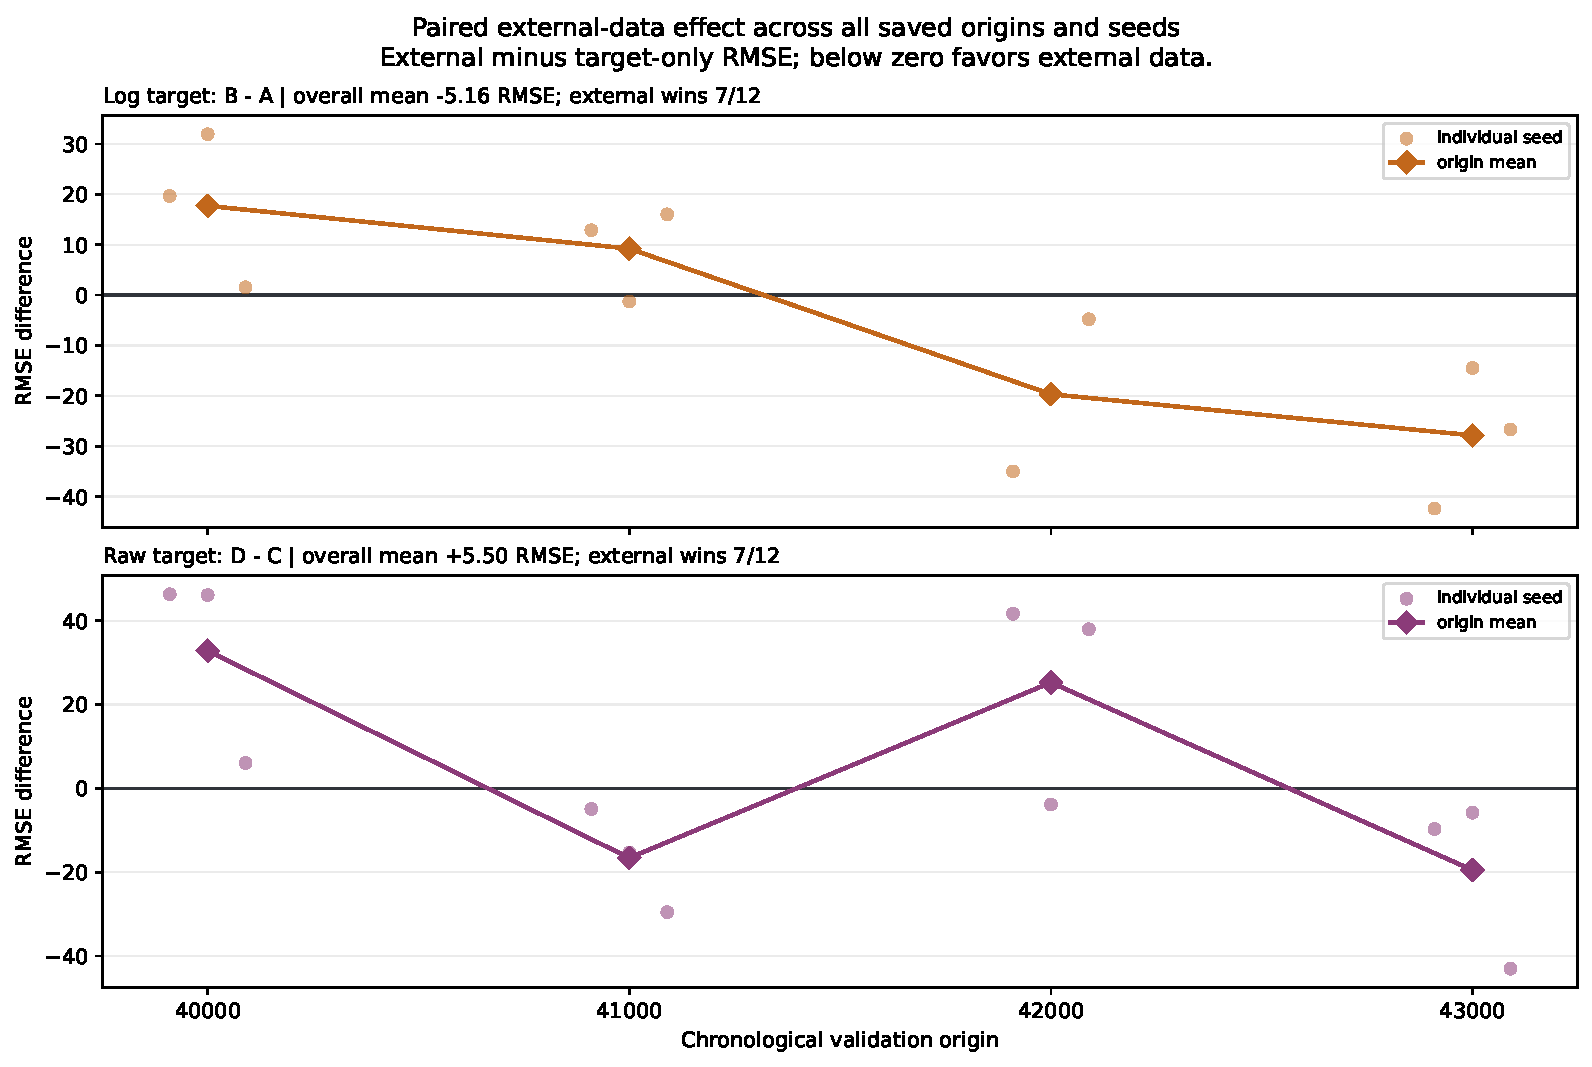
\includegraphics[width=\linewidth]{figures/q2_ablation_rmse.pdf}
\caption{Change in RMSE after adding external data for matched runs. Dots
show individual seeds, diamonds show the average at each forecast starting
point. Values below zero mean external data helped.}
\label{fig:q2-ablation-rmse}
\end{figure}

\begin{figure}[ht]
\centering
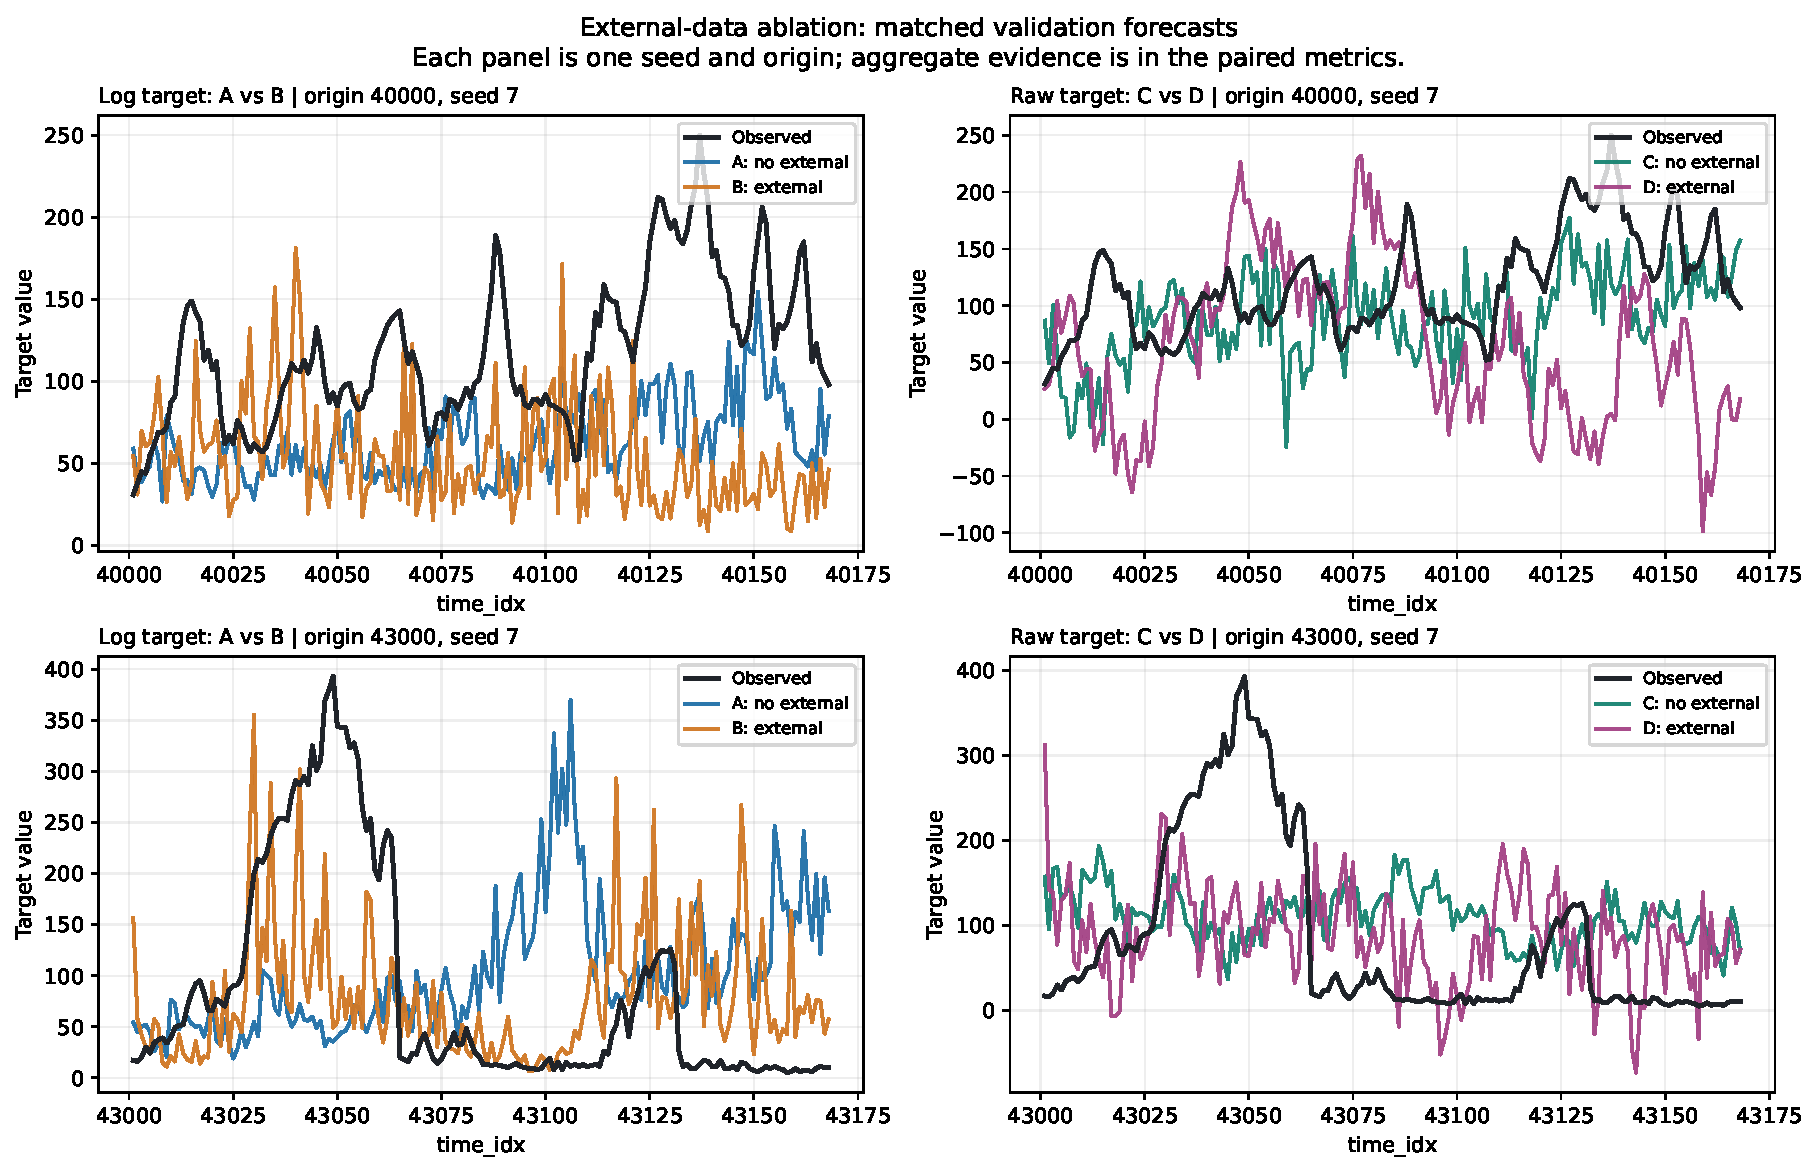
\includegraphics[width=\linewidth]{figures/q2_ablation_forecasts.pdf}
\caption{Actual values and forecasts for both external-data comparisons at
starting points 40000 and 43000, using seed 7. Tables
\ref{tab:q2-results} and \ref{tab:q2-ablation} summarize all runs.}
\label{fig:q2-ablation-forecasts}
\end{figure}

\clearpage
\subsection*{Forecast choice and limits}

We chose C, which trains on the raw target without external data, to predict
the next 168 values. Across the four validation starting points, it has the
lowest average MAE, RMSE, and sMAPE. It also uses 651 fewer parameters than B
or D and has the smallest RMSE variation across seeds. This choice is based
on validation results. At the latest starting point, B actually did better than C.Their average
RMSE values were 104.949 and 128.481.

For C, the middle value among the 12 selected best epochs was epoch 4.
We therefore trained a new C model with seed 7 for four epochs using all
43,656 observed values. It produced 168 ordered forecast values, all valid
numbers. The forecast comes from one model.
The model has $P=2{,}176{,}464$ trainable parameters and its final training
run used $E=4$ epochs. Two predicted values are negative, even though the
measured target is nonnegative. 


\section*{AI Usage}
I prompted AI to help with writing the forecasting implementations in notebook 1 and question 2. 
The plotting scripts were also written using AI assistance that I ran to generate the figures.

\end{document}
